\documentclass{article}

\usepackage{amsmath, mathrsfs, amssymb, stmaryrd, cancel, relsize,tikz,amsthm}
\usepackage[all]{xy}
\theoremstyle{plain}
\newtheorem{theorem}{Theorem}[section]{\bfseries}{\itshape}
\newtheorem{proposition}[theorem]{Proposition}{\bfseries}{\itshape}
\newtheorem{definition}[theorem]{Definition}{\bfseries}{\upshape}
\newtheorem{lemma}[theorem]{Lemma}{\bfseries}{\upshape}
\newtheorem{corollary}[theorem]{Corollary}{\bfseries}{\upshape}
\newtheorem{exercise}[theorem]{Exercise}{\bfseries}{\upshape}

\theoremstyle{definition}
\newtheorem{example}[theorem]{Example}{\bfseries}{\upshape}

\newcommand{\tvs}{\textvisiblespace}
\newcommand{\ra}{\rightarrow}
\newcommand{\la}{\leftarrow}
\newcommand{\co}{\mathbf{code}}

\title{ITCS 532 Foundations of Computer Science\\
Class 6 - Tractability and $p$-Time Reduction}
\author{Rob Egrot}
\date{}

\begin{document}
\maketitle
\subsection{The Running Times of Algorithms}
So far in this course we have only asked whether decision problems are decidable or semidecidable. For this purpose we only care about the existence, or provable non-existence, of algorithms (modeled by Turing machines) for achieving particular tasks. By this measurement we have seen that, for example, Turing machines with multiple tapes are equivalent to standard Turing machines, because any decision problem that can be decided, or task that can be accomplished, by a multitape TM can be solved or accomplished by a machine with only one tape. 

We have made no distinction between algorithms that can be run on a home computer in less than a second, and algorithms that would take the most powerful supercomputers in the world billions of years to complete. In the real world though, it is actually quite important that our algorithms can be run in a `reasonable amount of time'. Computational complexity theory aims, among other things, to systematize the study of the running times of algorithms (and also their use of other computational resources such as memory), and formalize the concept of a `reasonable amount of time' as far as possible.

We want our measure of the running time of an algorithm to be independent of the hardware we run it on. It might take my desktop several hours to solve a problem that a supercomputer could solve in a few seconds, even if the computation uses the same algorithm. To get around this difficulty, we think about the number of steps involved in solving a problem. The idea is that each computational step takes a constant amount of time on each system, so even if the steps take different times on different systems, the total number of steps taken to run the same algorithm on the same input will be the same for all systems. We can think of these steps as being steps in a Turing machine computation, or, more practically, CPU cycles.

Another thing to consider is that we want our algorithms to run on \emph{inputs} (like our Turing machines have been doing), so the time an algorithm takes will depend on the input we give it. The idea is to represent the running time of an algorithm as a function of its input. Inputs are considered to be strings over a finite alphabet, and we know the set of these strings is countably infinite. It's not practical for us to give a precise function assigning a number to each possible input for a halting computation (its run time), so we simplify by looking for a function of the \emph{length} of the input. 

However, we have another problem because inputs of the same length may have different run times. To get around this we traditionally think about the worst case. I.e. what is the slowest possible (halting) run time of this algorithm for an input of length $n$? This will give us a function of $n$, e.g. $f(n)=4n^3-5n +6$. In this example, $f$ tells us that given an input of size $n$ the largest possible number of steps our algorithm can take to complete its run is $4n^3-5n +6$. So, for example, the algorithm will always be finished within 28 steps if the input has length 2. We only care about successful computations here, so we ignore the possibility of inputs not properly corresponding to instances of the problem we're trying to solve causing the algorithm to run forever.

The final difficulty is that the function which tells us the longest possible halting computation on an input of length $n$, while well defined mathematically (as there are only a finite number of inputs of each length), will usually not have a neat description such as in our polynomial example. To address this issue we introduce the idea of a function being \emph{bounded} by another function. So, for example, the function we're interested in may be too complicated to describe, but if we know it's bounded by a simple function we have useful information about its behaviour. The following definition makes this precise. 

\begin{definition}[Big $O$ Notation]
Let $f$ and $g$ be functions from $\mathbb{R}$ to $\mathbb{R}$, and suppose $g(x)$ is strictly positive for large enough values of $x$ (i.e. after some point the values of $g(x)$ are all bigger than zero). We say $f=O(g)$ as $x\ra\infty$ if there are $x_0,c\in\mathbb{R}$ such that $|f(x)|\leq cg(x)$ for all $x\geq x_0$. 
\end{definition}

We use big $O$ notation to roughly classify the running times of algorithms. For example, if $f(n)=4n^3-5n +6$ then $f=O(n^3)$. Intuitively this tells us that, once $n$ gets big enough, the value of $f(n)$ will be bounded above by $cn^3$, for some constant $c$. This gives us a rough measure of the worst case run time of $f$. We are mainly interested in finding algorithms whose big $O$ worst case run time is as small as possible, as this sets an upper bound on the worst possible performance. Note that in the real world sometimes we are more interested in average case performance. For example, \emph{Quicksort} has a worst case run time of $O(n^2)$, but worst case behaviour is rare, and the algorithm usually runs in $O(n\log(n))$. 

The following diagram (taken from the Wikipedia page for Big $O$ notation) illustrates the growth rates some common functions used in big $O$ notation. 

\[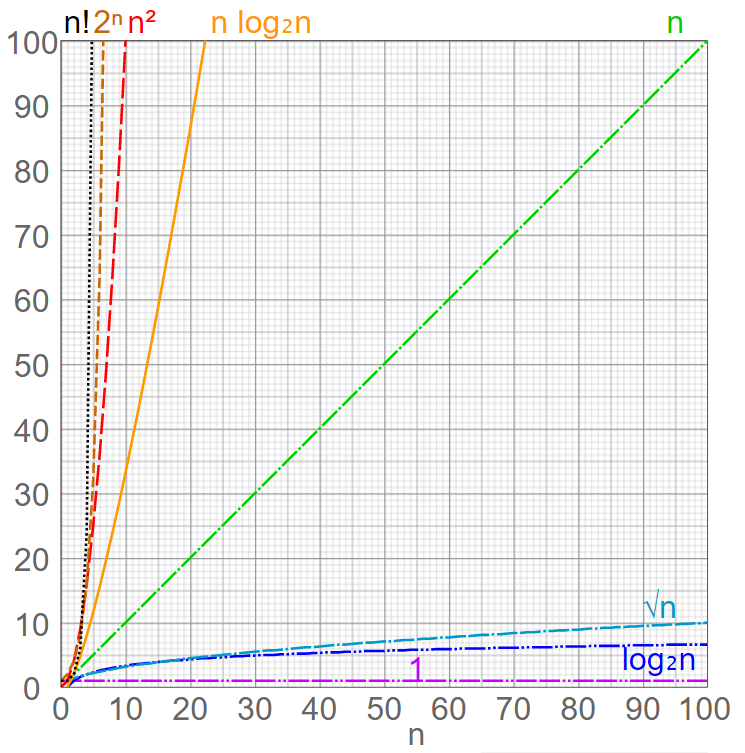
\includegraphics[width= 0.6\textwidth]{comp.png} \]             


\subsection{Algorithm Efficiency vs. Computer Power}
Computers are improving all the time, and tasks that would take hours on the earliest computers can be done in seconds today. However, these improvements primarily apply to algorithms that are relatively efficient. As the run time complexity (represented by its big $O$ class) of an algorithm gets worse, the effect of an increase in raw computation power becomes less significant. 

The first thing to understand is that the problems with inefficient algorithms come up when the input size is relatively large. For very small inputs, for example, the worst case time complexity of an `inefficient' algorithm might be better than that of an `efficient one'. We generally don't consider this to be important from a theoretical standpoint, because for small enough inputs our computers just blast through the problems basically whatever algorithm we use (so long as it's not ridiculous). What happens with inefficient algorithms is that as the input size increases they quickly `hit a wall', and a small increase in the size of the input suddenly results in a very large increase in the running time of the algorithm. 

This increase means you can go from `computations that can be done in a few seconds' to `computations that take hours or days' just by increasing the input size a little bit. So when we think about computing power for inefficient algorithms, what we want to know is, ``how much bigger can we make the input before the computation time becomes unreasonable?". Of course, people building real computers also care about linear increases in efficiency too, because running an algorithm in half the time can be a big difference in practice, but from the `broad strokes' theory standpoint we don't consider it.      

Anyway, suppose we have an algorithm for solving a given decision problem, suppose we have computers $C_1$ and $C_2$ running this algorithm, and suppose finally that $C_2$ is capable of performing $2^{12}$ computation steps in the time it takes $C_1$ to do 1 (so $C_2$ is 4096 times faster than $C_1$ - in symbols $v_2 = 2^{12}v_1$, where $v_i$ is the number of computation steps machine $C_i$ can take each second). How much improvement does this give us in terms of the size of inputs that can be computed in the same time? The answer depends on the running time of the algorithm. 

Suppose first that the algorithm runs in linear time (i.e. $f$ is $O(n)$, where $f$ is the `worst case run time' function we talked about before). Let $t$ be some fixed amount of time (in seconds). The maximum number of steps it takes $C_1$ to run the algorithm on an input of length $n_1$ is given by $f(n_1)$, and $f(n_1)\leq cn_1$ for some constant $c$, as $f$ is $O(n)$. To guarantee that $C_1$ completes the computation in at most time $t$, we require that $cn_1\leq v_1t$, because $v_1t$ is the maximum number of computation steps $C_1$ can take in time $t$. Rearranging the formula, we must have $n_1\leq \frac{v_1t}{c}$. In other words, the largest input length for which we can guarantee $C_1$ will complete the algorithm within $t$ seconds is $\lfloor \frac{v_1t}{c}\rfloor$. What about $C_2$? 

To answer this, let $v_2$ be the number of computation steps $C_2$ takes every second. Remember that $v_2 = 2^{12}v_1$. Similar to the case of $C_1$, if we want to be sure $C_2$ completes the computation in at most $t$ seconds on an input of length $n_2$, we require $cn_2\leq v_2 t$, which rearranges to give $n_2\leq \frac{v_2t}{c}$. In other words, the largest input length for which we can guarantee $C_2$ will complete the algorithm within $t$ seconds is $\lfloor \frac{2^{12}v_1t}{c}\rfloor$. This is $2^{12}$ times bigger than for $C_1$, so is a huge improvement.

What happens when the algorithm has worse performance? Suppose now the algorithm runs in quadratic time (i.e. $f(n)$ is $O(n^2)$, so $f(n)\leq cn^2$ for some constant $c$). Let $v_1$ and $v_2$ be as before. This time, to guarantee completion in at most time $t$ by $C_1$ on an input of length $n_1$, we must have $cn_1^2\leq v_1t$. In other words, $n_1\leq \sqrt{\frac{v_1t}{c}}$. Similarly, for $C_2$, we must have input length \[n_2\leq \sqrt{\frac{v_2t}{c}}=\sqrt{\frac{2^{12}v_1t}{c}}= 2^6\sqrt{\frac{v_1t}{c}}.\]   
In other words, roughly speaking, the biggest input guaranteed to halt within $t$ seconds on $C_2$ is $2^6$ times bigger than the biggest such input for $C_1$. Another big improvement, but significantly worse than in the linear case.

Suppose now we have a really inefficient algorithm that runs in exponential time (i.e. $f$ is $O(2^n)$). Then we have $2^{n_1}\leq \frac{v_1t}{c}$ and $2^{n_2}\leq \frac{v_2 t}{c}$ for some constant $c$, and by taking logs base 2 this gives $n_1\leq \log(v_1) + \log(t) - \log (c)$, and $n_2\leq \log(v_2) + \log(t) - \log (c)$.
Since $v_2=2^{12}v_1$, the second inequality can be rewritten as 
\begin{align*}n_2&\leq \log(2^{12}v_1) + \log(t) - \log (c)\\
&= \log(2^{12}) +\log(v_1) + \log(t) - \log (c)\\
&= 12 + \log(v_1) + \log(t) - \log (c).\end{align*}
This tells us that the biggest input guaranteed to halt within $t$ seconds on $C_2$ is only 12 bigger than the biggest such input for $C_1$. Not 12 times, just plus 12. This is a very small improvement considering how much faster $C_2$ is than $C_1$. The lesson from this is that faster hardware cannot do much to compensate for truly inefficient algorithms.    


\subsection{Tractability and Intractability}
Complexity theory divides algorithms into rough complexity classes based on their use of resources. We're interested in run time, so the classes we discuss here are based on worst case run time as discussed previously. We've seen how we can define the worst case run time of an algorithm as a function of the size of its input, and we've also introduced big $O$ notation to group algorithms into classes based on the upper bounded run time of their fastest know algorithm (e.g. $O(n)$, $O(n^3)$, $O(2^n)$ etc.). The difference between $O(n^2)$ and $O(n^3)$ is actually very important in applications. For example, in some applications an $O(n^3)$ algorithm might be much too slow, but an $O(n^2)$ algorithm might be manageable. For some applications, e.g. in Big Data, $O(n^2)$ might be much too slow. Despite this, theorists often make a sharp distinction between  `efficient' and `inefficient' algorithms, and between `easy' and `hard' decision problems, based on the following definitions.

\begin{definition}[polynomial time]
An algorithm is polynomial time ($p$-time) if it is $O(n^k)$ for some $k\in\mathbb{N}$.
\end{definition}

\begin{definition}[tractable]
A decision problem is tractable if there is a polynomial time algorithm that decides it. It is \emph{intractable} otherwise. 
\end{definition}

As a rough approximation, complexity theorists consider tractable problems to be `easy', and intractable ones to be `hard'. In practice, a polynomial time algorithm might be much too slow for practical use, as mentioned above. Of course, finding a polynomial time algorithm for a problem, thus demonstrating its `easiness', may not be easy at all!


\subsection{Run Time Vs. Encoding System}
The question of whether a given $n\in\mathbb{N}$ is prime is a simple and important decision problem. Consider the following algorithm:

\begin{verbatim}
Prime(n).

answer = `true'
for i = 2 to n-1
	if i divides n then answer = `false'
return answer.	
\end{verbatim} 

Testing if $i$ divides $n$ is quite fast. Say we have an $O(n^2)$ algorithm for this (just calculate $ij$ for every $1< j\neq i < n$ - I'm not claiming this is the best possible run time for this algorithm). The the worst case running time of the `Prime' algorithm would be $O(n^3)$, as we check if $i$ divides $n$ for every $i$ between $2$ and $n$. However, if we want to run this algorithm on a Turing machine we need to encode natural numbers using a finite alphabet, and the length of the input is the number of symbols we use, not the size of the number. For example, a binary number of length $n$ can represent a natural number up to $2^n-1$. So considered as a function of binary input length this algorithm has a worst case run time of $O((2^n)^3)=O(2^{3n})$, because the length $n$ input might correspond to the number $2^n-1$.  

On the other hand, if we use unary notation then the algorithm does indeed run in $p$-time, as then the length of the input is equal to the size of the number. What this tells us is that there is a relationship between how we encode problems and the running times of algorithms we can use to solve them. We can make algorithms look more efficient by representing the problem in an inefficient way. This is somewhat similar to the relationship between the complexity of encoding systems for Turing machines and the minimum size of universal Turing machines that can simulate them. There we can trade higher complexity of encoding for smaller size of minimal UTM and vice versa. By the way, you shouldn’t take the details of the calculations above too seriously as we were loose with our treatment of the algorithm for checking divisibility, but hopefully the main point is clear.  

It turns out that there are $p$-time algorithms for (binary) primality testing, for example the $AKS$ test, but these use some number theory tricks, and their run times are too slow to be practical in most applications (roughly, a little slower than $O(\log(n)^6)$). In industry people generally use probabilistic algorithms based on mathematical number theory for primality testing. These are much faster, but don't always give the correct answer (though errors can be made very rare).     


\subsection{Polynomial Time Reduction}
Previously we saw how we can order decision problems in terms of their decidability using reduction. That is, $A\leq B$ if there's an algorithm that turns `yes' instances of $A$ into `yes' instances of $B$, and `no' instances of $A$ into `no' instances of $B$. The notation comes from the fact that, if such an algorithm exists, then we could use an algorithm for solving $B$ to solve $A$ too, so problem $B$ is `at least as hard' as problem $A$.

We can extend the idea of reduction to order decision problems in terms of their polynomial time solvability. We write $A\leq_p B$ if there is a $p$-time algorithm that turns `yes' instances of $A$ into `yes' instances of $B$, and `no' instances of $A$ into `no' instances of $B$. Then, if we had a $p$-time algorithm for solving $B$ we could combine it with the $p$-time conversion algorithm to get a $p$-time algorithm for solving $A$.

Actually there is a complication here. Our first algorithm converts instances of $A$ to instances of $B$ in $p$-time, and the second algorithm solves $B$ in $p$-time. But the second algorithm runs in $p$-time on the size of its input, and the algorithm that converts instances of $A$ to instances of $B$ does not necessarily preserve their sizes. So, if the first algorithm dramatically increases the size of an instance of $A$ while converting it then, even though the second algorithm runs in $p$-time on the converted input, we might worry that it could end up running slower than $p$-time on the size of the original instance of $A$. 

Fortunately, this is not a problem because the fact that the conversion algorithm is $p$-time bounds the size of the converted instance. I.e. if the conversion algorithm runs in time $n^k$ for some $k$ and the original $A$ instance has size $m$, then the converted instance can be at most size $cm^k$ for some constant $c$. Then, if the algorithm for solving $B$ is $O(n^l)$ for some $l$, the worst case run time for converting this instance of $A$ to an instance of $B$ then solving with the algorithm for $B$ is $O((n^k)^l)=O(n^{kl})$, which is $p$-time.    

\begin{exercise}
Why is it obvious that $\leq_p$ is reflexive?
\end{exercise}

\begin{theorem}
$\leq_p$ is transitive.
\end{theorem}
\begin{proof}
Suppose $A\leq_p B$ and $B\leq_p C$. If $I$ is an instance of $A$ let $f(I)$ be the result of applying the reduction of $A$ to $B$ to $I$. Similarly, if $J$ is an instance of $B$ let $g(J)$ be the result of applying the reduction of $B$ to $C$ to $J$. We can compose $f$ and $g$ as functions, so $g(f(I))$ is a reduction of $A$ to $C$. We need to check $g\circ f$ is $p$-time. Suppose the reduction of $A$ to $B$ is $O(n^k)$ for some $k$, and the reduction from $B$ to $C$ is $O(n^l)$ for some $l$. Then the maximum size of $f(I)$ is $O(n^k)$, so $g\circ f$ is $O((n^k)^l)=O(n^{kl})$. So $g\circ f$ is $p$-time as required.
\end{proof}

\begin{theorem}\label{T:Pmin}
Let $A$ and $B$ be decision problems. Then, if there is a $p$-time algorithm for solving $A$, and if $B$ has at least one `yes' instance and at least one `no' instance, then $A\leq_p B$.
\end{theorem}
\begin{proof}
Since there's a $p$-time algorithm for solving $A$, to convert instances of $A$ to instances of $B$ we just use the $p$-time algorithm to check if they are `yes' or `no' instances of $A$ then convert them to either the `yes' or `no' instance of $B$ appropriately. This `conversion' is constant time,  as we always convert to either the fixed `yes' instance, or the fixed `no' instance. 
\end{proof}

We know that $\leq_p$ is not symmetric, because if $\leq_p$ were symmetric it would follow from theorem \ref{T:Pmin} that every decision problem would have a $p$-time solution. Since there are problems that are not even decidable this is impossible. However, we can use $\leq_p$ to define a relation between decision problems that is reflexive, transitive, and symmetric (i.e. an equivalence relation).

\begin{definition}[$\equiv_p$]
Decision problems $A$ and $B$ are \emph{$p$-time equivalent} if $A\leq_p B$ and $B\leq_p A$.
\end{definition} 


\subsection{Example - The Hamiltonian Circuit Problem and the Traveling Salesman Decision Problem}
We consider two decision problems and show that one is $p$-time reducible to the other.

\begin{definition}[Hamiltonian circuit] 
Given a finite simple graph $G$ with $n$ vertices, a Hamiltonian circuit is a sequence $c=(v_1,v_2,\ldots,v_n)$ such that
\begin{enumerate}
\item if $v_i$ and $v_j$ occur consecutively in the sequence then there is an edge from $v_i$ to  $v_j$ in $G$,
\item every vertex of $G$ occurs in $c$, and
\item there is an edge from $v_n$ to $v_1$.  
\end{enumerate}  
\end{definition}

Informally a Hamiltonian circuit is a path in $G$ that passes through every vertex exactly once before returning to its origin.

\begin{definition}[$HCP$]
The Hamiltonian circuit problem ($HCP$) is whether a given finite undirected simple graph has a Hamiltonian circuit.
\end{definition}

\begin{definition}[weighted graph]
A weighted graph is a graph where every edge is associated with a number (usually a non-negative integer). This number can be thought of as the `cost' of traveling along that edge.
\end{definition}

\begin{definition}[$TSDP$]\label{D:TSDP}
The traveling salesman decision problem ($TSDP$) has instances $(G,d)$, where $G$ is a finite complete undirected weighted simple graph with non-negative integer weights, and $d$ is a non-negative integer. The question is whether there is a Hamiltonian circuit in $G$ such that the sum of the weights of the edges used in the circuit is less than or equal to $d$. 
\end{definition}

\begin{theorem}\label{T:TSDPtoHCP}
$HCP\leq_p TSDP$, where the reduction is $p$-time when considered as a function of the number of vertices plus the number of edges of the instance graph $G$.
\end{theorem}
\begin{proof}
An instance of $HCP$ is a finite undirected simple graph $G$ with $n$ vertices and $e$ edges. We will convert $G$ into a pair $(G',d)$ where $G'$ is a finite complete undirected weighted simple graph, and $d$ is a non-negative integer. This is an instance of $TSDP$. We then show that `yes' instance of $HCP$ become `yes' instances of $TSDP$, and similar for `no' instances. Finally we check that the conversion algorithm runs in $p$-time as a function of $n+e$.

Let $G'$ have the same vertices as $G$. To be an instance of $TSDP$ $G'$ must be complete, so we add edges for pairs of vertices. We now weight the edges so that the edges between vertices that are connected by an edge in $G$ have weight 0, and the rest have weight $1$. We set $d=0$. So $G'$ has a Hamiltonian circuit with total weight 0 if and only if there is a Hamiltonian circuit in $G$ (because the edges with weight 0 in $G'$ are precisely the edges of $G$). This shows the reduction is correct.

How fast is the reduction? Well, we have to clone the vertices of $G$. Assuming it takes constant time to clone a single vertex, doing this for every vertex will take linear time. I.e. $O(|V|)$, where $V$ is the set of vertices of $G$. Then we add edges for pairs of vertices. There are $n \choose 2$ pairs of vertices of $G$, so assuming it takes constant time to add a single edge, doing this for every pair takes quadratic time. I.e. $O(|V|^2)$. Setting the weights involves checking every edge of $G'$ to see if it corresponds to an edge of $G$. We can do this naively just by checking every edge of $G$ to see if it is an edge between $v$ and $v'$ for every pair $v,v'\in V$. This is $O(|E|\times|V|^2)$, where $E$ is the set of edges of $V$. Finally, setting $d=0$ is a constant time operation, say $c$. So the whole process takes $O(|V|)+O(|V|^2)+O(|E|\times|V|^2)+c$, which is $O((|V|+|E|)^3)$ at most. This is $p$-time as required.  
\end{proof}

The converse to the theorem above is also true. If you are feeling ambitious you can try to prove it directly using $p$-time reduction. This direction is harder than the direction proved in the theorem. We will prove it using some powerful general theory at the end of the course.



\end{document}